% $Header: /home/vedranm/bitbucket/beamer/solutions/conference-talks/conference-ornate-20min.en.tex,v 90e850259b8b 2007/01/28 20:48:30 tantau $

\documentclass{beamer}

% This file is a solution template for:

% - Talk at a conference/colloquium.
% - Talk length is about 20min.
% - Style is ornate.



% Copyright 2004 by Till Tantau <tantau@users.sourceforge.net>.
%
% In principle, this file can be redistributed and/or modified under
% the terms of the GNU Public License, version 2.
%
% However, this file is supposed to be a template to be modified
% for your own needs. For this reason, if you use this file as a
% template and not specifically distribute it as part of a another
% package/program, I grant the extra permission to freely copy and
% modify this file as you see fit and even to delete this copyright
% notice. 


\mode<presentation>
{
  \usetheme{AnnArbor}
  % or ...

  \setbeamercovered{transparent}
  % or whatever (possibly just delete it)
}


\usepackage[francais]{babel}
% or whatever

\usepackage[utf8]{inputenc}
% or whatever

\usepackage{times}
\usepackage[T1]{fontenc}
% Or whatever. Note that the encoding and the font should match. If T1
% does not look nice, try deleting the line with the fontenc.


\title % (optional, use only with long paper titles)
{Apprentissage profond et représentation latente de séquences peptidiques}

\author{Rémy Sun} % (optional, use only with lots of authors)

\institute[ENS Rennes] % (optional, but mostly needed)
{
  Département d'informatique\\
  ENS Rennes
}
% - Use the \inst command only if there are several affiliations.
% - Keep it simple, no one is interested in your street address.

\date[XTRA 2016] % (optional, should be abbreviation of conference name)
{XTRA 2016}
% - Either use conference name or its abbreviation.
% - Not really informative to the audience, more for people (including
%   yourself) who are reading the slides online

\subject{Theoretical Computer Science}
% This is only inserted into the PDF information catalog. Can be left
% out. 



% If you have a file called "university-logo-filename.xxx", where xxx
% is a graphic format that can be processed by latex or pdflatex,
% resp., then you can add a logo as follows:

% \pgfdeclareimage[height=0.5cm]{university-logo}{university-logo-filename}
% \logo{\pgfuseimage{university-logo}}



% Delete this, if you do not want the table of contents to pop up at
% the beginning of each subsection:
\AtBeginSubsection[]
{
  \begin{frame}<beamer>{Outline}
    \tableofcontents[currentsection,currentsubsection]
  \end{frame}
}


% If you wish to uncover everything in a step-wise fashion, uncomment
% the following command: 

%\beamerdefaultoverlayspecification{<+->}


\begin{document}

\begin{frame}
  \titlepage
\end{frame}

\begin{frame}{Outline}
  \tableofcontents[pausesections]
  % You might wish to add the option [pausesections]
\end{frame}


% Structuring a talk is a difficult task and the following structure
% may not be suitable. Here are some rules that apply for this
% solution: 

% - Exactly two or three sections (other than the summary).
% - At *most* three subsections per section.
% - Talk about 30s to 2min per frame. So there should be between about
%   15 and 30 frames, all told.

% - A conference audience is likely to know very little of what you
%   are going to talk about. So *simplify*!
% - In a 20min talk, getting the main ideas across is hard
%   enough. Leave out details, even if it means being less precise than
%   you think necessary.
% - If you omit details that are vital to the proof/implementation,
%   just say so once. Everybody will be happy with that.

\section{Apprentissage profond?}

\subsection{Pourquoi l'apprentissage \og profond\fg?}

\begin{frame}{Fonctionnement d'un neurone}
  % - A title should summarize the slide in an understandable fashion
  %   for anyone how does not follow everything on the slide itself.

  \begin{columns}
    \column{0.38\linewidth}
    \begin{figure}
      \centering
      
\includegraphics[scale=0.17]{../Figures/Neuron}
    \end{figure}

    \column{0.5\linewidth}
    \begin{itemize}
    \item Entrée $A$, poids $W$, biais $b$
    \item Transformation linéaire $WA + b$\pause
    \item Activation non-linéaire $f$\pause
    \item Evaluation (score) de la sortie \pause
    \item Apprentissage de $W$ et $b$ par rétropropagation sur le score
    \item Réseau neuronal: plusieurs neurones en parralléle
    \end{itemize}
  \end{columns}

\end{frame}

\begin{frame}{Du réseau de neurones au réseau de neurones profonds}
  % - A title should summarize the slide in an understandable fashion
  %   for anyone how does not follow everything on the slide itself.

  \begin{columns}
    \column{0.5\linewidth}
    \begin{figure}
      \centering
      \includegraphics[scale=0.1750]{../Figures/Deep}
    \end{figure}

    \column{0.4\linewidth}
    \begin{itemize}
    \item Plusieurs couches de neurones \pause
    \item Hiérarchie: plusieurs niveaux de représentations \pause
    \item Evanouissement de gradient \pause
    \item Grands ensembles d'entraînement \pause
    \end{itemize}
  \end{columns}

\end{frame}

\subsection{Entraînement non-supervisé}

\begin{frame}{Fixer une cible  de manière autonome}
  % - A title should summarize the slide in an understandable fashion
  %   for anyone how does not follow everything on the slide itself.

  \begin{columns}
    \column{0.45\linewidth}
    \begin{figure}
      \centering
      \includegraphics[scale=0.8]{../Figures/DenseAuto}
    \end{figure}

    \column{0.5\linewidth}
    \begin{itemize}
    \item Non supervisé\pause
    \item Encodage\pause
    \item Représentation latente \pause
    \item Décodage \pause
    \item Eviter d'encoder l'identité\pause
      \begin{itemize}
      \item Compression\pause
      \item Bruitage\pause
      \item Régularisation
      \end{itemize}
    \end{itemize}
  \end{columns}
\end{frame}

\subsection{Architectures standards}

\begin{frame}{Réseaux Convolutionnels: recherche de caractéristique}
  % - A title should summarize the slide in an understandable fashion
  %   for anyone how does not follow everything on the slide itself.

    \begin{figure}
      \centering
      \includegraphics[scale=0.5]{../Figures/CNN}
    \end{figure}

    \begin{itemize}
    \item Filtres de caractéristiques\pause
    \item Permet d'isoler des caractéristiques locales\pause
    \end{itemize}
\end{frame}

\begin{frame}{Réseaux récurrents: tenir compte de l'ordre d'apparition}
  % - A title should summarize the slide in an understandable fashion
  %   for anyone how does not follow everything on the slide itself.
  \begin{columns}
    \column{0.4\linewidth}
    \begin{figure}
      \centering
      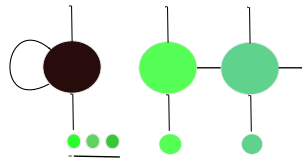
\includegraphics[scale=0.15]{../Figures/Recurrent}
    \end{figure}

    \column{0.5\linewidth}
    \begin{itemize}
    \item Dépendance temporelles\pause
    \item Sortie + état caché persistant (boucle de rétroaction)\pause
    \item Pas de dépendances hiérarchiques\pause
    \item Réseau \og profond\fg à une couche \pause
    \item Très utilisé en langages naturels\pause
    \item Unité LSTM (Long Short-Term Memory)
    \end{itemize}
  \end{columns}
\end{frame}

\begin{frame}{Eviter le sur-entraînement}
  % - A title should summarize the slide in an understandable fashion
  %   for anyone how does not follow everything on the slide itself.

  \begin{columns}
    \column{0.5\linewidth}
    \begin{figure}
      \centering
      \includegraphics[scale=0.3]{../Figures/dropout}
    \end{figure}

    \column{0.45\linewidth}
    \begin{itemize}
    \item Désactiver aléatoirement des neurones\pause
    \item Eliminer la concentration d'information\pause
    \item Faire travailler tout le réseau\pause
    \item Généraliser la représentation apprise\pause
    \item Permet d'entraîner ad nauseam
    \end{itemize}
  \end{columns}
\end{frame}

\subsection{Application: Protéines}

\begin{frame}{Plus qu'une chaîne d'acides aminés}
  % - A title should summarize the slide in an understandable fashion
  %   for anyone how does not follow everything on the slide itself.
  \begin{figure}
    \centering
    \includegraphics[scale=0.3]{../Figures/prot}
  \end{figure}
    \begin{itemize}
    \item Acide aminés: molécules chimiques\pause
    \item Structure primaire: chaîne d'acides amminés\pause
    \item Structure secondaire: structures locales formé par les acides\pause
    \item Structure tertiaire: forme tridimensionnelle \pause
    \end{itemize}
\end{frame}

\subsection{Etat de l'art}

\begin{frame}{Peu de travaux concernant les protéines}
  % - A title should summarize the slide in an understandable fashion
  %   for anyone how does not follow everything on the slide itself.

      \begin{itemize}
      \item Succés en:\pause
        \begin{itemize}
        \item Reconnaissance d'image, langages naturels,
          prédiction de sentiments, données bio-médicales,
          représentation, ...\pause
        \end{itemize}
      \end{itemize}


      \begin{itemize}
      \item Protéines:
        \begin{itemize}
        \item Prédiction de structures secondaires\pause
          \begin{itemize}
          \item H. R, P. K, L. J 2015 Improving prediction of secondary
            structure, local backbone angles, and solvent accessible surface
            area of proteins by iterative deep learning. \pause
          \item S. M, E. J, C. J. 2015 A Deep Learning Network Approach to ab
            initio Protein Secondary Structure Prediction\pause
          \end{itemize}
        \item Classification de protéines selon différents critéres\pause
          \begin{itemize}
          \item H. S, H. M, O. K. Fast model-based protein homology detection
            without alignment. 2007 \alert{1 seule couche récurrente}\pause
          \end{itemize}
        \item Prédiction de contacts
          \begin{itemize}
          \item L. PD, N. K, B. P. 2012 Deep architectures for protein contact
            map prediction. \pause
          \end{itemize}
        \end{itemize}
      \end{itemize}


\end{frame}

\section{Etude réalisée}

\subsection{Séquences peptidiques}

\begin{frame}{Traiter les protéines à partir de la structure primaire}
  % - A title should summarize the slide in an understandable fashion
  %   for anyone how does not follow everything on the slide itself.

    \begin{itemize}
    \item Tâche sur une chaîne longue: prédiction de classe structurale\pause
      \begin{itemize}
      \item Découpage de la chaîne en fragments courts
      \end{itemize}
    \item Travaux usuels: représentation par pseudo-vecteur de fréquence des protéines\pause
    \item Etude sur les séquences peptidiques\pause
    \item Représentation de l'acide $a_i$ par $V = (v_k)$ où $v_i = 1$ et $v_k =
      0 (k\ne i)$
    \end{itemize}
\end{frame}

\subsection{Architectures entrainées}

\begin{frame}{Autoencodeurs}
  % - A title should summarize the slide in an understandable fashion
  %   for anyone how does not follow everything on the slide itself.

  \begin{columns}
    \column{0.35\linewidth}
    \begin{figure}
      \centering
      \includegraphics[scale=0.1]{../Figures/Class}
      \caption{Carte de corrélation entre représentation latente et propriétés connues}
    \end{figure}

    \column{0.6\linewidth}
    \begin{itemize}
    \item Entraînement sur des fragments de taille 11\pause
    \item Augmentation de la taille de l'ensemble d'entraînement\pause
    \item Encodeur \alert{récurrent}\pause
    \item Décodeur récurrent
    \end{itemize}
  \end{columns}
  
\end{frame}

\begin{frame}{Classificateur de classe structurales}
  % - A title should summarize the slide in an understandable fashion
  %   for anyone how does not follow everything on the slide itself.

  \begin{columns}
    \column{0.45\linewidth}
    \begin{figure}
      \centering
      \includegraphics[scale=0.135]{../Figures/Class}
    \end{figure}

    \column{0.5\linewidth}
    \begin{itemize}
    \item Tâche: classifier les classes structurales des protéines\pause
    \item Classificateur convolutionnel\pause
    \item Premières couches pré-entraînées\pause
    \item Validation de la représentation latente acquise
    \end{itemize}
  \end{columns}

 \end{frame}

\subsection{Résultats}

\begin{frame}{Les représentation latentes présentent des corrélations remarquables}
  % - A title should summarize the slide in an understandable fashion
  %   for anyone how does not follow everything on the slide itself.

  \begin{columns}
    \column{0.5\linewidth}
    \begin{figure}
      \centering
      \includegraphics[scale=0.1650]{../Figures/SingleOneRecHeat}
      \caption{Carte de corrélation entre représentation latente et propriétés connuesphysico-chimiques}
    \end{figure}

    \column{0.4\linewidth}
    \begin{itemize}
    \item Dimensions liées dans l'espace latent\pause
    \item Corrélation de coordonnées à l'hydropathie, à la charge ...\pause
    \item Pas de corrélation à la structure secondaire observées\pause
    \end{itemize}
  \end{columns}

\end{frame}

\begin{frame}{Les représentations latentes sont exploitables par un
    classificateur structural}
  % - A title should summarize the slide in an understandable fashion
  %   for anyone how does not follow everything on the slide itself.

    \begin{itemize}
     
    \item Comparaison favorable au même classificateur non pré-entrainé:
      \begin{itemize}
      \item Atteinte plus rapide de la précision maximale\pause
      \item Précision maximale plus élevée\pause
      \end{itemize}
    \item Pertinence de la représentation latente\pause
    \end{itemize}

 \end{frame}

\begin{frame}{Pistes de recherche}
  % - A title should summarize the slide in an understandable fashion
  %   for anyone how does not follow everything on the slide itself.

    \begin{itemize}
    \item Architectures d'auto-encodeurs à attention\pause
    \item Acquisition d'une représentation pertinente des acides aminés\pause
    \item Etude plus approfondie des hyper-paramètres\pause
    \item Hiérarchiser les caractéristiques à utiliser en apprentissage\pause
    \item Initialisation couche par couche?
    \end{itemize}
 \end{frame}


\section*{Conclusion}

\begin{frame}{Résumé}

  % Keep the summary *very short*.
  \begin{itemize}
  \item
    L'apprentissage profond permet de \alert{détecter des structure
      hiérarchiques ou temporelles}.\pause
  \item
    Problème particulier: Peu \alert{d'exemples labélisés} et \alert{chaînes très longues}.\pause
  \item
    Apparition de \alert{corrélations} entre la représentation latente et des
    caractéristiques des séquences peptidiques.\pause
  \end{itemize}
  
  % The following outlook is optional.
  \vskip0pt plus.5fill
  \begin{itemize}
  \item
    Perspectives\pause
    \begin{itemize}
    \item
      Utilisation d'autres architectures utilisée en langages naturels.\pause
    \item
      Influence des hyper paramètres.
    \end{itemize}
  \end{itemize}
\end{frame}



% All of the following is optional and typically not needed. 
\appendix
\section<presentation>*{\appendixname}
\subsection<presentation>*{For Further Reading}

\begin{frame}[allowframebreaks]
  \frametitle<presentation>{For Further Reading}
    
  \begin{thebibliography}{10}
    
  \beamertemplatebookbibitems
  % Start with overview books.

  \bibitem{Author1990}
    A.~Author.
    \newblock {\em Handbook of Everything}.
    \newblock Some Press, 1990.
 
    
  \beamertemplatearticlebibitems
  % Followed by interesting articles. Keep the list short. 

  \bibitem{Someone2000}
    S.~Someone.
    \newblock On this and that.
    \newblock {\em Journal of This and That}, 2(1):50--100,
    2000.
  \end{thebibliography}
\end{frame}

\end{document}
